% !TEX TS-program = XeLaTeX

\documentclass[12pt, notitlepage,
draft
]{ctexbook}
\usepackage{xeCJK}
\usepackage[font=small]{caption, subcaption}
\usepackage{tikz}
\usepackage{fancyhdr}
\usepackage{amsmath}
\usepackage{graphicx}
\usepackage{xcoffins}
\usepackage{xcolor}
\usepackage{fontspec}
\usepackage[a4paper]{geometry}
\usepackage{setspace}
\usepackage{emptypage}
\usepackage{titlesec}
\usepackage[breaklinks,colorlinks,linkcolor=black,citecolor=black,urlcolor=black]{hyperref}
% Set up commands for title page generation
\definecolor{ethblue}{RGB}{31, 64, 122}


\newfontfamily\dinprobold{HBLiXuKeShuFa}
\newCJKfontfamily\cnprobold{HBLiXuKeShuFa}
\newCJKfontfamily\cnproregular{HBLiXuKeShuFa}
\newCJKfontfamily\cnprolight{KaiTi}
\graphicspath{ {images/} }
\newcommand\chapterdecoration{%
	\begin{tikzpicture}[remember picture,overlay,shorten >= -10pt]
	\filldraw[black,line width=0,rounded corners=0] (0,2.5) rectangle (\linewidth,2.55);
	\end{tikzpicture}%
}
\titleformat{\chapter}[display]%
{\heiti\zihao{1}}%
{第\zhnumber\thechapter 章}{10pt}%
{}[\vspace*{2cm}\chapterdecoration]

\begin{document}

	\pagestyle{empty}
	\NewCoffin \result
\NewCoffin \anchor
\NewCoffin \topbox
\NewCoffin \ethlogo
\NewCoffin \imagebox
\NewCoffin \textbox
\NewCoffin \departmentlogo
\NewCoffin \textboxtext
\NewCoffin \textboxsubtext
\NewCoffin \authortext

\SetHorizontalCoffin \result {}
\SetHorizontalCoffin \topbox {\color{ethblue}\rule{220mm}{3cm}}
\SetHorizontalCoffin \imagebox {\includegraphics[width=190mm]{haupt}}
%\SetHorizontalCoffin \ethlogo {\includegraphics[width=50mm]{ethlogo}}
\SetHorizontalCoffin \textbox {\color{ethblue}\rule{190mm}{100mm}}
\SetVerticalCoffin \textboxtext {160mm} {\fontsize{60}{72}\cnprobold\noindent\textcolor{white}{\dinprobold{CDAI} 文化指南}}
\SetVerticalCoffin \textboxsubtext {160mm} {\fontsize{21}{25}\cnproregular\noindent\textcolor{white}{——中德文化差异小百科}}
\SetVerticalCoffin \authortext {160mm} {\flushright\fontsize{10}{12}\cnprolight\noindent\textcolor{white}{中德工程师学院}}
\SetHorizontalCoffin \departmentlogo {\includegraphics[width=30mm]{logo}}

% Positioning Hax
\JoinCoffins \result \topbox
\JoinCoffins \result[\topbox-hc, \topbox-b] \imagebox [hc, t](0mm,10mm)
\JoinCoffins \result[\imagebox-l, \imagebox-t] \ethlogo [l, b](0mm,5mm)
\JoinCoffins \result[\imagebox-l, \imagebox-b] \textbox [l, t](0mm,0mm)
\JoinCoffins \result[\textbox-hc, \textbox-t] \textboxtext [hc, t](-5mm, -5mm)
\JoinCoffins \result[\textboxtext-l, \textboxtext-b] \textboxsubtext [l, t](0mm, -5mm)
\JoinCoffins \result[\textbox-r, \textbox-b] \authortext [r, b](-5mm, 5mm)
\JoinCoffins \result[\textbox-l, \textbox-b] \departmentlogo [l, t](-5mm, -5mm)


% Generate the page
\thispagestyle{empty}
\newgeometry{left=0mm,bottom=0mm, top=0mm, right=0mm}
\noindent\TypesetCoffin \result
\restoregeometry
	\cleardoublepage
	\thispagestyle{empty}
	\begin{titlepage}
	\centering
	%\vspace*{8cm}
	\noindent
	\center
	\begin{minipage}{\linewidth}
	%\zihao{0}\heiti CDAI文化指南\par
	\fontsize{60}{72}\cnprobold{\dinprobold{CDAI}文化指南}\par
	\vspace{12pt}
	%\zihao{-2}\songti ——中德文化差异百科\par
	\fontsize{21}{25}\cnproregular{——中德文化差异小百科}\par
	\vspace{8cm}
	\heiti\zihao{-3}
	%\includegraphics{logo}
	\raggedright
	项目成员:\\
	
	\vspace*{1em}
	\zihao{4}
	黄伟根\\
	黄耀鑫 \hspace{1em} 杨星林 \hspace{1em} 詹均升 \\
	张嘉伟 \hspace{1em} 周功豪 \hspace{1em} 周鹏 \\
	\end{minipage}
	\vfill
	\zihao{3}\cnprolight{中德工程师学院}\par
	\href{http://cdai.zust.edu.cn/}{\texttt{http://cdai.zust.edu.cn/}}
	\end{titlepage}

	\cleardoublepage
	\vspace*{3cm}
\begin{minipage}{\linewidth}
    \Huge\heiti\center{封面图片} \par
\end{minipage}

 \vspace*{3cm}

\par
勃兰登堡门位于德国首都柏林的市中心,最初是柏林城墙的一道城门,因通往勃莱登堡而得名。现在保存的勃莱登堡门是一座古典复兴建筑,由普鲁士国王腓特烈·威廉二世下令于1788年至1791年间建造,以纪念普鲁士在七年战争取得的胜利。
\cleardoublepage

\begin{minipage}{\linewidth}
\Huge\heiti\center{关于本书} \par
\end{minipage}

\vspace*{3cm}
 %\normalfont\normalsize
 %\raggedright
 %\indent
中国和德国都是世界上具有重大影响力的国家,随着传播 通讯技术的改进,交通技术的进步和经济的高度全球化,两国的合作越来越频繁。 然而,由于文化背景的不同,中德两国人民在文化交流上还略有欠缺。针对中德工程师学院和德国的应用技术大学之间日益频繁的交流活动,作为中德工程师学院的学生我们希望将一些所闻所知的信息整理、归类,尽可能为两国的学生了解对方文化提供一些一些帮助。本书不求包罗万象,但求准确,详尽,有趣。

\par
在上学期,我们小组成员在项目发起人Frau Schneider的引领和指导下,为了增进我院及合作院校中、德两国学生间的文化认同感,减轻乃至消除文化差异所带来的沟通障碍,同时也为了我院新生能够更快适应和融入国际化的教学方式,多元化的人文环境,开展了一系列关于中德文化差异的研讨会、采访、问卷调查和现场调研。我们最终决定将项目的视角聚焦在七个文化主题上:服饰、饮食、体育、工作、交通、文化、卫生,以Wiki为载体,配以百科全书式的写作手法,从学生的视角出发,独特地展现出我们对于异国文化的认识与思考。在项目期间,我们充分运用所学项目管理的知识,通过Projekt Auftrag, Zeitplan, PSP等项目管理工具精确的控制项目进程;通过查阅相关资料、与德国师生互相交流讨论,并结合实际的生活体验,确定了各项主题的具体内容,并定期向同学与老师展示工作成果。项目的最后,我们的成果是喜人的,我们的中德文化差异百科全书在学院官网上线,向中德师生展现了中德文化大花园的一隅,虽然项目仍有不少改进的空间,但是我们希望通过这个学期的共同努力,把中德文化差异百科这座文化桥梁打造的更加坚固、优美。 相比于上学期, 这学期我们将从中德两国人民的日常行为差异入手,深入分析每个差异代表的文化内涵。我们希望通过这些方法,使中德两国国学生增进理解,弥合文化差异的鸿沟。
\par
在中国有一个小故事,讲的是汉朝的时候,在西南方有个名叫夜郎的小国家,它虽然是一个独立的国家,可是国土很小,百姓也少,物产更是少得可怜。但是由于邻近地区以夜郎这个国家最大,从没离开过国家的夜郎国国王就以为自己统治的国家是全天下最大的国家。有一天,夜郎国国王与部下巡视国境的时候,他指着前方问说:“这里哪个国家最大呀?”部下们为了迎合国王的心意,于是就说:“当然是夜郎国最大啰!”走着走着,国王又抬起头来、望着前方的高山问说:“天底下还有比这座山更高的山吗?”部下们回答说:“天底下没有比这座山更高的山了。”后来,他们来到河边,国王又问:“我认为这可是世界上最长的河川了。”部下们仍然异口同声回答说:“大王说得一点都没错。”从此以后,无知的国王就更相信夜郎是天底下最大的国家。有一次,汉朝派使者来到夜郎,途中先经过夜郎的邻国滇国,滇王问使者:“汉朝和我的国家比起来哪个大?”使者一听吓了一跳,他没想到这个小国家,竟然无知的自以为能与汉朝相比。却没想到后来使者到了夜郎国,骄傲又无知的国王因为不知道自己统治的国家只和汉朝的一个县差不多大,竟然不知天高地厚也问使者:“汉朝和我的国家哪个大?”。夜郎国王固然可笑,但如果我们固步自封坐井观天岂不是跟夜郎国王一样。
\par
在如今全球化的背景下,中国青年更应该睁眼看世界,走出国门拥抱世界。德国作为世界上数一数二的大国。德国文化更是不可忽视的。面对中德两国日益平凡的交流,德国青年对中国文化越来越有兴趣。总之,这本小册子希望可以作为两国学生了解对方文化的起点。作为中国学生我们对德国文化没有更深入的了解,在此也欢迎正在看此书的你,提出宝贵的建议。
\par
\vspace{\baselineskip} 
\hfill {\heiti 2019年三月,杭州}

	\tableofcontents

	\pagestyle{headings}	
	\input{Essen/Essen}
	\chapter{节日文化差异}
在德国提到节日可以说“Fest”、“Festival”以及“Feiertag”,对应中国的来说可以是节日和法定假日,“Festival”一般是在某个城市或小镇举办的音乐节或是狂欢节。对于中国人来说法定假日的数量不多,更多的是拼假组成的黄金周。
\input{Festival/Traditionelles_Festival}
\section{政治性节日}

\subsection{马丁·路德宗教改革日}

每年10月31日,五个德国州聚集在一起庆祝宗教改革日。随着这个国家动荡而微妙的历史,人们可能会想知道庆祝的是哪个改革活动,或者为什么只有大约三分之一的国家在庆祝。旨在回答这些问题以及更多问题,这里有一段德国宗教改革日的简史。宗教改革日是观察新教改革的官方公共假日,由德国僧侣马丁·路德颁布。具体来说,德国的宗教改革日标志着他在1517年将他著名的95篇论文钉在维滕贝格教堂门口的周年纪念日。他在11月1日万圣节前夕这样做,因为他知道许多人会聚集在教堂,这确保了他的论文的最大可见性。路德最感兴趣的是废除出售赎罪券作为寻求赎罪的手段。在路德的时代,众所周知,这笔钱被用来资助罗马圣彼得大教堂的翻修,这说明了出售放纵品的做法有多腐败。然而,95篇论文列出了路德对教会怀有的许多其他不满。这一重大事件给德国和其他国家带来了重大变化,因为路德教和其他新教派别开始反对天主教会,在这些抗议活动发生时,天主教会确实变得相当专制。当路德用拉丁文写这些论文时,这些论文被迅速翻译成德语,并在全国和其他地方广泛传播。改革时期在随后的一个世纪里以重要的社会、历史和宗教方式进行,直到1648年。宗教改革浪潮中出现了多个新教教派,教会在人民生活中调解上帝存在的作用受到了彻底的审视。早在1567年,各个教派的新教教会每年秋季都举行一天的活动,纪念95篇论文的发表。然而,在当代,在大多数地方,宗教改革日是在10月31日。每年,德国的州一级都会庆祝这个节日。包括勃兰登堡州、萨克森州、梅克伦堡西波美拉尼亚州、图林根州和萨克森安哈尔特州在内的五个州是该国宗教改革日为官方假日的地方。这五个州在历史上都是新教徒,在95篇论文发表后,社会和文化生活发生了重大变化。今天,这些地区通过给人们放假来纪念宗教改革日。此外,为纪念这一天,银行和邮局等公共机构也关闭了。在这些地方和其他地方,路德教会和改革派教会经常举行特别纪念活动。用来代表这一天的象征性颜色是红色,这是针对圣灵的。赞美诗《强大的堡垒是我们的上帝》通常是为了向写这首诗的路德致敬而唱的。为了纪念路德,许多面包、蛋糕和甜食也在这一天传统上被消费。

马丁·路德宗教改革出现的根本原因是随着西欧商品经济和资本主义的发展,天主教会成为资本主义发展的最大障碍,专制君主、银行家和商人、中小贵族、新兴资产阶级、下层贫民,都想通过反对教会来改善自己的经济状况。对德国的影响有推动了广大民众的反封建斗争,沉重打击了天主教会和封建势力,有利于德意志民族语言的发展,并为欧洲的其他国家和地区的宗教改革开辟了道路。那么在宗教改革日那天德国人会做些什么呢?每年10月31日,五个德国州聚集在一起庆祝宗教改革日。随着这个国家动荡而微妙的历史,人们可能会想知道庆祝的是哪个改革活动,或者为什么只有大约三分之一的国家在庆祝。旨在回答这些问题以及更多问题,这里有一段德国宗教改革日的简史。宗教改革日是观察新教改革的官方公共假日,由德国僧侣马丁·路德颁布。具体来说,德国的宗教改革日标志着他在1517年将他著名的95篇论文钉在维滕贝格教堂门口的周年纪念日。包括勃兰登堡州、萨克森州、梅克伦堡西波美拉尼亚州、图林根州和萨克森安哈尔特州在内的五个州是该国宗教改革日为官方假日的地方。今天,这些地区通过给人们放假来纪念宗教改革日。此外,为纪念这一天,银行和邮局等公共机构也关闭了。在这些地方和其他地方,路德教会和改革派教会经常举行特别纪念活动。用来代表这一天的象征性颜色是红色,这是针对圣灵的。赞美诗《强大的堡垒是我们的上帝》通常是为了向写这首诗的路德致敬而唱的。为了纪念路德,许多面包、蛋糕和甜食也在这一天传统上被消费。

\paragraph{马丁·路德的故事}
路德在1517年万灵节前夕,也就是十月三十一日那天,宣布他反对赎罪券,写了九十五条论纲。其实这九十五条的目的并非是号召宗教改革,只是路德以一位大学教授的身份将赎罪券的神学提出来讨论罢了。路德反对赎罪券的曲解和误用,这不但对人的得救不利,还影响了教会的正常运作。当时的人们认为天国的钥匙在教会手里,一个人进入天堂前要先洗清生前所犯的一切罪行。他们最怕的是死后在炼狱中的刑罚,因此他们相信只要用赎罪券就可以上天堂,一张赎罪卷能缩短死后在炼狱中的刑罚。而赎罪劵可以在教堂里购买,因此当时的教堂和牧师都很有钱。马丁路德发现这样的说法与作法完全不能见容于圣经与理性。赎罪券的买卖鼓励了处于罪恶中的人,不去思想基督,不去祈求上帝的饶恕。就这一点,路德的神学与天主教会的神学有明显的不同。1530年路德在奥斯堡会议上为新运动作了解释,他的改教运动已把基督教欧洲一分为二,更正教会产生了三个主要路线:信义宗、改革宗和英国圣公宗。更正教会主张信徒应该直接和基督联合,因为基督是救恩的唯一来源。他的救恩借着圣灵的能力和上帝的道的教导,临到悔改的信徒。路德的宗教改革受到四面攻击。罗马教廷要路德收回他的言论和著作,路德并没有答应。在他隐居于瓦尔特堡(Wartburg)那段日子里,路德把整本新约圣经由希腊文译成精彩的德文。在那期间,左派极端的社会行动到处兴事,路德于是回到威登堡以稳定大学和教会的生活,并且应付四面八方涌来的攻击。甚至有的人民误解了路德说的自由,牵扯到政治,拿了武器去争取,造成了改教运动的致命伤。路德被罗马教会定罪,逐出教会。
\begin{figure}[htb]
    \centering
    
\includegraphics[width=0.6\linewidth]{mdld}
    \caption{马丁路德}
    
\end{figure}

\subsection{妇女节}

创立国际劳动妇女节的主要提议者:克拉拉·蔡特金(Clara Zetkin,1857.7.5-1933.6.20),原名克拉拉·艾斯纳,德国社会民主党和第二国际左派领袖之一,国际社会主义妇女运动领袖之一,德国共产党创始人之一,无产阶级女权解放的灵魂人物。1910年8月,蔡特金在丹麦首都哥本哈根召开了国际社会主义者第二次妇女代表大会。倡议以每年的3月8日作为全世界妇女的斗争日,1911年的3月8日为第一个国际劳动妇女节。“三八”妇女节成为世界妇女争取权利、争取解放的节日。

在德国柏林地区,妇女节是法定假期,全天休假。

\subsubsection{妇女节在中国 ——三八红旗手}
是中国在三月八号妇女节颁给优秀劳动妇女的荣誉称号,主要是表彰在中国各条战线上为社会主义物质文明和精神文明建设做出显著成绩的妇女先进人物和妇女先进集体

\paragraph{政治背景}
中华人民共和国成立后,鼓励妇女进入工厂工作,离开传统的家庭区。 它们主要被视为工作的来源,因此是一个在文化领域,特别是当时的政治宣传方面出现充满力量感的女性形象。
\begin{figure}[htb]
    \centering
    \includegraphics[width=0.3\linewidth]{frau1}
    \includegraphics[width=0.3\linewidth]{frau2}
    
    \includegraphics[width=0.3\linewidth]{frau3}
    \includegraphics[width=0.3\linewidth]{frau4}
    \caption{中国曾经的政治宣传画}
\end{figure}
\input{Festival/Regionales_Festival}
\section{节日禁忌} 
\begin{figure}[htb]
    \centering
    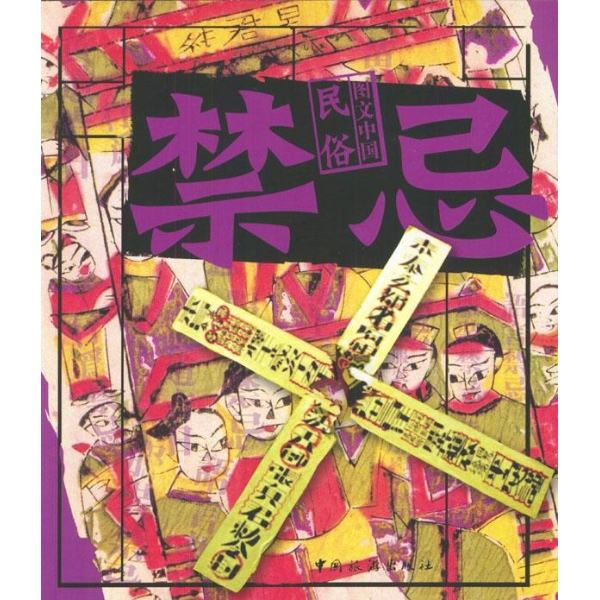
\includegraphics[width=0.5\linewidth]{jinji}
    \caption{节日禁忌}
    
\end{figure}

    “禁忌”一词来源于,国际学术界统称为“塔布”,源于太平洋小岛波利尼西亚汤加岛人的土语,音译为“taboo”或“Tabu”,其基本含义是表示“神圣的”、“不洁的”、和“危险的”、“不可接触的”。
    中国文化博大精深,然而在中国的传统文化当中有很多的禁忌,如果按照老一辈的人来说,这是老天爷安排的。按照现代人说,这就是迷信。但是无论是迷信是否,作文中国文化,我们更应该用继承的心态去面对。下面就介绍一些中国人在日常生活中碰到的或是不愿意去犯的禁忌。



\subsection{送礼禁忌}

    相信不止大家都为了挑选礼物而烦恼过,面对各种各样的节日,我们总是需要不停的购买适当的礼物送给对应的人,这个真的很让人苦恼。但是亲朋好友之间互相送礼物,更多的是为了传达一种祝福、表达一种诚意。用最近火热的词来说,就是一种“仪式感”。你挑选的礼物不一定真的符合你送礼对象的心意,或者也不是他们真正需要的。给同样的钱让他们自己买他们或许也不会买这个礼物,甚至你礼物送出去之后他们一辈子都不一定会用上一次。然而你在挑选礼物的过程中,已经投入了大量的精力和时间,而正是这些东西,会让对方感受到你的心意,这就是所谓的“礼轻情意重。”所以但是根据中国的风俗传统,送以下系类的礼物却可能会导致好心做坏事,也是众多礼物中比较忌讳的礼物:

    \begin{enumerate}
   \item 
   送结婚礼物时忌讳送“伞”、“钟”等物,因为“伞”与“散”谐音,散意离散,为人们所不喜欢,所以伞被视为不吉利的礼物,“钟”与“终”谐音,特别是“送钟”更会让老人们联想到“送终”,很不吉利。
   \item
   给病人送食品时也有谐音的禁忌。旧时上海去看望病人时,忌送苹果,因为上海话中“苹果”的发音与“病故”谐音。
   \item
   菊花常用于纪念逝者,不可以作为礼物送出。
   \item
   帽子俗话中有“愁帽子”之说,老人去世孝子要头戴孝帽,所以忌讳将帽子送给别人。特别是绿色的帽子,更是送礼的大忌。
   \item
   刀剑等利器,容易伤人,且俗话有“一刀两断”之说,用于送人恐有割断关系双方的不好联想,所以一般不作为礼品送人。
   \item
   扇子因为只用于夏天,一到秋凉天即被抛之不用,有绝情之意,俗称“送扇无相见”,所以不受欢迎,而且很多人会将“风扇”当成“分散”理解,潜台词就是分手。
   \item
   “鞋”与“邪”同音,而且鞋被踩在脚下,所以除了自己家人,一般不要给别人送鞋。
   \begin{figure}[htb]
    \centering
    
\includegraphics[width=0.5\linewidth]{jinjifs}
    \caption{禁忌风水}
    
    \end{figure}
   \item
   ”梨“因为“梨”与“离”谐音,给夫妻、恋人不能送就很不适合。
   \item
   “镜子”与“禁子”谐音,且镜子易破易碎,所以也属于属送礼的忌讳之物。
   
  
        
    \end{enumerate}


\subsection{数字禁忌}

    数字不仅仅可以代表数量,还关联着不同语言文化、宗教信仰等深刻内涵。不同的国家地区都有着不同的数字禁忌,也有着不一样的数字偏好。如中国人就忌讳4,偏爱6、8、9。
    \begin{enumerate}
    \item 
    “四”谐音“死”,大凶,所以门牌号、车牌号都不宜有这个数字。过年的时候也忌说“4”、“死”等音的词。在日常生活中也能看到这样的例子:有很多外国人在中国生活久了之后都清楚在中国绝大部分大厦中是没有“4楼”的存在,通常是用“3A楼”或者“5A楼”来代替,或者直接就没有这一层楼,直接跳到了5楼。。这也是因为在中国的文字发音中间“4”和“死”同音,中国人普遍都忌讳死亡楼层。
    \item 
    数字当中,最吉利的要数六和八,所谓“六六大顺”、“要得发,不离八”,就说出了其中的原委。  
        
    \end{enumerate}
\begin{figure}[htb]
    \centering
    \includegraphics[width=0.6\linewidth]{4_Echt}
    \caption{中国常见的楼层分布}
\end{figure}


\subsection{谐音产生的禁忌}

    每年春节,全世界有超过十亿人加入庆祝的行列,并展开一场微妙的文字游戏。它很像一组求爱仪式——为了招来好运,人们会用喜庆字样的剪纸来装点住宅与门户。要理“发”的,年前赶紧理完,谁想在新年伊始削去财运,哪怕只是稍事修剪?年夜饭的菜肴里通常有鱼,因为人们希望“年年有余”;有的地方还时兴吃一种名为发菜的藻类,因为谐音“发财”;或有“橙”,寓意为“成”,所以在春节的装饰物中常常可以看见柑橘类水果的身影。而且有研究表明,在中文语境下,人们对同音歧义似乎更为敏感。
    \begin{enumerate}
    \item 
   如在亲友结婚之日,忌讳说“死、光、输、完、离、散、休”等不吉利字词。
   \item 
   在结婚时,新娘上门禁吃瓜类,因为“瓜”与“寡”谐音,以免将来做寡妇。
   \item 
   和亲友一起吃梨时不能分吃一个梨,因为“分梨”与“分离”谐音。
   \begin{figure}[htb]
    \centering
    
\includegraphics[width=0.5\linewidth]{bagua}
    \caption{阴阳八卦:在中国阴阳八卦是所有禁忌产生的根源}
    
    \end{figure}

     
    

   \item 
   沿海渔民或船家忌说“沉”、“箸”等字。因为“沉”和“沉船”的沉同音同字,因此人们把“沉”字改说“重”字。吃饭用的“箸”与“住”谐音,即停住抛锚之意,对行船来说是不吉利的。因此人们把吃饭时用的“箸”改称“筷子”,取“筷”与“快”的谐音,即“快”行、“一帆风顺”之意。
   \item 
   在广州一带,人们把“猪舌”称作“猪月利”,由于广东话中“舌”与“蚀”同音,经商者忌讳蚀本,改称“猪月利”则含“月月盈利”的意思。北京话“舌”与“折”同音,也有“折本”不吉利之嫌,因此北京、天津等地把“猪舌”称作“口条”。广州人把丝瓜称作“胜瓜”,因为广州话“丝”与“输”谐音。广东潮汕一带把“药”称作“利市”或“甘茶”,而忌说“药”字,因为“药”与“病”相关,所以把有病“服药”叫“辗利市”或“服甘茶”。
        
    \end{enumerate}

\subsection{其他}

    除了上文中的禁忌之外,中国人在日常生活中还有许多有趣的禁忌。
    \begin{enumerate}
    \item
    \textbf{在中国写别人名字的时候十分忌讳用红笔书写}

   这一点在老一辈人中间特别在意,在他们看来红色墨水写出来的字颜色接近血色,是带有诅咒的意思,如果用红色墨水写一个人的名字将会给这个人带了厄运,所以很多的老师在小学的时候就会告诉小孩子不要用红笔写名字。

   \item
   \textbf{吃饭的时候所有人都忌讳将筷子竖拆在饭碗中间}

   第二个几乎是所有中国小孩都喜欢做的事情,但是无一例外都被家长斥责过。在中国是习惯吃米饭的,不像西方国家吃饭是都是使用刀叉,在中国使用的餐具基本上都是筷子,在吃饭的时候所有人都忌讳将筷子竖拆在饭碗中间,这种现象在别人看来几乎是和祭拜死人没什么差别,所有人都十分忌讳,除此之外也不能在吃饭的时候用筷子指着别人。

   \item
   \textbf{忌讳在家里种柳树}

   柳树,想必大家都很熟悉了,一种非常漂亮的树,一条条柳条随风飘摇。但是这种树虽然很好看,但是有没有小伙伴们注意到,这么漂亮的树一般很少出现在私人庭院或是哪个企业的庭院之中。因为从古至今,在民间人们都说,柳树是极阴之物,一般很少人会去接近柳树,即便是很好看也只是站在较远的地方观赏。正因为柳树是极阴之物,所以在夜晚甚至是白天的时候,会引得很多孤魂野鬼在柳树底下吸食阴气。如果有人在柳树底下呆久了,运气不好的话很有可能被冤鬼缠上,而且在阴气较重的地方呆久了,阴气入体,轻则大病一场,重则一命呜呼。也正是柳树是嫉阴之物,所以在古代民间很多道士或是先生那里都会准备一些柳条,因为柳条是可以直接抽鬼的,就像用鞭子抽人一样,有着驱鬼的功能。

   \item
   \textbf{不能敲饭碗}

   敲碗首先会显得没有教养。比如去别人家作客,假如敲碗,那么意思就是在催主人快点,等不及了。其次是民间有种说法,说吃饭敲碗,以后生活会不好,会出去乞讨,因为乞丐要饭才敲碗。
        
   \begin{figure}[htb]
    \centering
    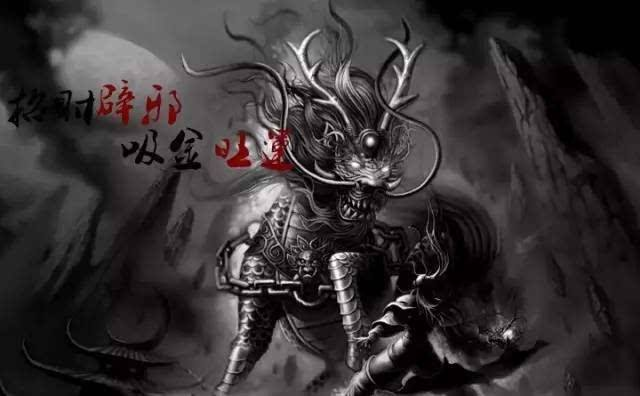
\includegraphics[width=0.5\linewidth]{qlbx}
    \caption{辟邪:中国人用它驱赶不吉利的事物}
    
    \end{figure}

    \end{enumerate}



   “十里不同风,百里不同俗”,在中国,各民族、各地区都有千姿百态的民俗。民俗是民间记忆的载体,反映了普通民众在历史长河中不断发展、变化的生产、生活情境以及蕴含在其中的精神与情感,是中国传统文化的重要组成部分。中国有五千年的历史,从迷信走到了科学,但是每个地方还是有老辈人口传下来的忌讳,如人的一生以36岁为大忌,每个人到了35就不做比较危险的工作,就是做什么事都比较小心点,一直到37就可以了,很多人连36这个数字都很忌讳,买卖东西不可以出现36,少给都可以,不然准挨骂,还有很多,譬如打牌的人不可以买红色的包包,过年吃团圆饭的时候严禁别人串门,又譬如一串很忌讳的老话,正月不见鹰打鸟,二月不见狗擦裆,三月不见蛇吸雾,四月不见人成双,就是看见了就会有灾难找上门。这些中国各地在不同期间的不同的习俗和禁忌,也是非常有趣又有意义的,这也是我们民族文化传统的一部份,值得世代流传。

	
\end{document}